\chapter{Metode Penelitian}
\label{ch3}

Bab ini menjelaskan metodologi yang digunakan dalam perancangan dan pengembangan sistem \textit{blockchain-based cooperative} Lakomi. Pembahasan mencakup pendekatan penelitian, alat dan bahan, alur penelitian, arsitektur sistem, desain \textit{smart contract}, desain \textit{frontend}, alur kerja sistem, serta strategi pengujian.

\section{Pendekatan Design Science Research}

Penelitian ini mengadopsi pendekatan \textit{Design Science Research} (DSR) yang berfokus pada perancangan dan evaluasi \textit{artefak} teknologi untuk mengatasi masalah praktis \cite{hevner2004design}. DSR dipilih karena penelitian bertujuan menghasilkan sistem \textit{proof of concept} yang memetakan 26 ketentuan UU 25/1992 ke dalam \textit{smart contract} yang dapat dieksekusi.

Pemilihan DSR sebagai metodologi penelitian didasarkan pada tiga pertimbangan utama. Pertama, DSR menekankan pada pembangunan \textit{artefak} sebagai kontribusi utama, dalam konteks ini, \textit{artefak} berupa empat \textit{smart contract} yang mengimplementasikan regulasi perkoperasian ke dalam kode yang dapat dieksekusi secara otomatis. Kedua, DSR bersifat iteratif dan memungkinkan evaluasi berkelanjutan, setiap fungsi \textit{smart contract} diuji secara fungsional untuk memverifikasi kepatuhannya terhadap pasal spesifik dalam UU 25/1992. Ketiga, DSR menyeimbangkan antara kontribusi praktis (sistem yang berfungsi) dan kontribusi teoretis (model pemetaan regulasi ke \textit{smart contract}), yang sesuai dengan posisi penelitian ini di persimpangan antara rekayasa perangkat lunak dan ilmu hukum. Peffers dkk. \cite{peffers2007design} mengembangkan metodologi DSR yang lebih terstruktur dengan enam tahapan, identifikasi masalah, penetapan tujuan, desain dan pengembangan, demonstrasi, evaluasi, dan komunikasi, yang menjadi kerangka acuan untuk alur penelitian enam tahap yang diterapkan dalam penelitian ini.

Hevner \cite{hevner2007design} mengemukakan tiga siklus DSR, relevansi, rigor, dan desain, yang diterapkan sebagai berikut:

\begin{enumerate}
	\item Siklus Relevansi, Menjembatani lingkungan masalah dengan aktivitas penelitian. Siklus ini mengidentifikasi permasalahan koperasi tradisional, tata kelola tidak transparan, pengelolaan manual, partisipasi anggota terbatas, dan kesenjangan regulasi pengawasan~\cite{antoni2024permasalahan,putra2025dualisme}, serta kesenjangan antara DAO berbasis \textit{token-weighted voting} dengan prinsip koperasi satu-anggota-satu-suara. Hasil dari siklus relevansi adalah spesifikasi kebutuhan sistem yang diturunkan langsung dari UU 25/1992: 26 ketentuan yang harus diterjemahkan ke dalam fungsi \textit{smart contract} yang dapat diverifikasi.

	\item Siklus Rigor, Menjembatani basis pengetahuan ilmiah dengan aktivitas penelitian. Siklus ini mengkaji literatur tentang blockchain untuk koperasi, tata kelola DAO, regulasi perkoperasian Indonesia (UU 25/1992, PP 7/2021, Permenkop 8/2023), dan standar pengembangan \textit{smart contract}. Basis pengetahuan juga mencakup spesifikasi teknis Ethereum (Yellow Paper), standar ERC-20, pola desain keamanan \textit{smart contract} (AccessControl, ReentrancyGuard), dan arsitektur DChain sebagai infrastruktur blockchain konsorsium. Setiap keputusan desain dalam \textit{smart contract}, dari pemilihan basis poin SHU hingga ambang kuorum 67\%, dijustifikasi melalui rujukan ke regulasi atau literatur yang relevan.

	\item Siklus Desain, Membangun dan mengevaluasi \textit{artefak} secara iteratif. \textit{Artifact} yang dibangun berupa empat \textit{smart contract} (LakomiToken, LakomiVault, LakomiGovern, LakomiLoans) dan \textit{frontend} React. Evaluasi dilakukan melalui pengujian fungsional berbasis skenario yang memverifikasi setiap ketentuan UU 25/1992. Umpan balik dari hasil pengujian digunakan untuk memperbaiki implementasi secara iteratif hingga seluruh 26 ketentuan terverifikasi. Siklus desain menghasilkan dua artefak utama: (1) sistem \textit{proof of concept} yang berfungsi, dan (2) matriks pemetaan ketentuan hukum ke fungsi kode yang dapat digunakan sebagai acuan untuk pengembangan sistem serupa.
\end{enumerate}

Ketiga siklus DSR tidak berjalan secara linear, melainkan saling terkait secara dinamis. Temuan dari pengujian fungsional (siklus desain) dapat memicu pengkajian ulang terhadap literatur (siklus rigor), misalnya, ketika hasil pengujian menunjukkan bahwa suatu pola akses kontrol perlu diperkuat. Sebaliknya, literatur baru tentang regulasi perkoperasian (siklus rigor) dapat memperluas cakupan kebutuhan sistem (siklus relevansi). Interaksi dinamis antar siklus ini memastikan bahwa \textit{artefak} yang dihasilkan tidak hanya berfungsi secara teknis, tetapi juga memiliki justifikasi ilmiah dan relevansi praktis yang kuat.

\subsection{Justifikasi Ilmiah Data dan Evaluasi dalam DSR}

Berbeda dengan penelitian kuantitatif yang mengandalkan sampel data statistik (misalnya, pengujian hipotesis pada dataset di penelitian \textit{machine learning}), DSR mengevaluasi kebenaran \textit{artefak} terhadap spesifikasi yang telah ditetapkan, bukan terhadap populasi data. Dalam penelitian ini, spesifikasi yang menjadi acuan adalah 26 ketentuan operasional UU 25/1992, PP 7/2021, dan Permenkop 8/2023. Setiap ketentuan hukum bersifat diskret dan deterministik, suatu pasal baik dipenuhi atau tidak dipenuhi, tidak ada derajat kepatuhan parsial yang memerlukan inferensi statistik.

Data utama dalam penelitian ini adalah hasil verifikasi fungsional terhadap 26 skenario pengujian yang masing-masing menghasilkan luaran biner (Lulus/Gagal). Seluruh 26 skenario menunjukkan hasil Lulus, yang membuktikan bahwa \textit{artefak} memenuhi spesifikasi secara lengkap tanpa memerlukan generalisasi statistik. Data sekunder berupa 11 pengukuran konsumsi gas (45.969 sampai 245.599 gas per operasi) berfungsi sebagai bukti kelayakan operasional (\textit{utility}), bukan sebagai sampel yang mewakili populasi tertentu. Hevner~\cite{hevner2004design} menegaskan bahwa evaluasi dalam DSR cukup menunjukkan bahwa \textit{artefak} bekerja sesuai tujuannya (\textit{utility}) dalam konteks yang ditentukan, tanpa memerlukan validasi statistik terhadap populasi general.

\section{Alat dan Bahan}

\subsection{Perangkat Lunak}

Perangkat lunak yang digunakan dalam pengembangan sistem terdiri dari komponen \textit{smart contract}, \textit{frontend}, dan infrastruktur pendukung, sebagaimana dirangkum dalam Tabel~\ref{tab:alat-lunak}. Pengembangan dan pengujian awal dilakukan pada lingkungan lokal menggunakan Anvil (\textit{local Ethereum node}) sebelum di-\textit{deploy} ke jaringan DChain untuk pengujian integrasi dan evaluasi akhir.

\begin{table}[H]
\centering
\caption{Perangkat Lunak yang Digunakan}
\label{tab:alat-lunak}
\small
\begin{tabular}{p{0.22\textwidth}p{0.25\textwidth}p{0.12\textwidth}p{0.31\textwidth}}
\toprule
\textbf{Kategori} & \textbf{Nama} & \textbf{Versi} & \textbf{Kegunaan} \\
\midrule
\multirow{4}{*}{\textit{Smart Contract}} & Solidity & 0.8.20 & Bahasa pemrograman \textit{smart contract} \\
 & Hardhat & 2.22 & \textit{Framework} pengembangan, pengujian, dan \textit{deployment} \\
 & OpenZeppelin Contracts & 5.0 & Library standar (ERC-20, AccessControl, ReentrancyGuard) \\
 & Ethers.js & 6.x & Interaksi dengan jaringan EVM \\
\midrule
\multirow{3}{*}{\textit{Frontend}} & React & 18 & Framework antarmuka pengguna \\
 & TypeScript & 5.x & Bahasa pemrograman dengan \textit{type safety} \\
 & wagmi & 2.x & Library React Hooks untuk interaksi \textit{wallet} \\
\midrule
\multirow{3}{*}{Infrastruktur} & DChain &, & Jaringan blockchain konsorsium (EVM-compatible, Chain ID 17845) \\
 & Anvil &, & \textit{Local Ethereum node} untuk pengembangan dan pengujian awal \\
 & MetaMask &, & \textit{Wallet} browser untuk interaksi pengguna \\
\bottomrule
\end{tabular}
\end{table}

\subsection{Perangkat Keras}

Perangkat keras yang digunakan dalam pengembangan dan pengujian sistem adalah komputer dengan sistem operasi Ubuntu 22.04, prosesor Intel Core i7, memori 16 GB, dan koneksi internet untuk akses jaringan blockchain.

\subsection{Bahan Penelitian}

Bahan penelitian yang digunakan meliputi:

\begin{enumerate}
	\item Undang-Undang Nomor 25 Tahun 1992 tentang Perkoperasian sebagai acuan regulasi utama.
	\item Peraturan Pemerintah Nomor 7 Tahun 2021 tentang Kemudahan, Pelindungan, dan Pemberdayaan Koperasi dan UMKM.
	\item Peraturan Menteri Koperasi dan UKM Nomor 8 Tahun 2023 tentang Usaha Simpan Pinjam oleh Koperasi.
	\item Dokumentasi teknis Ethereum, Hardhat, OpenZeppelin, dan React sebagai acuan implementasi.
\end{enumerate}

\section{Alur Penelitian}

Penelitian dilaksanakan dalam enam tahapan yang diilustrasikan pada Gambar~\ref{fig:alur-penelitian}. Tahapan ini disusun dalam kerangka tiga siklus DSR: Relevansi (studi literatur dan identifikasi kesenjangan), Desain (perancangan arsitektur, implementasi smart contract, dan implementasi frontend), serta Rigor (pengujian fungsional dan evaluasi kepatuhan). Setiap tahapan menghasilkan luaran yang menjadi masukan bagi tahapan berikutnya, mencerminkan sifat iteratif dari metodologi DSR. Uraian rinci setiap tahapan disajikan setelah diagram alur.

\begin{figure}[H]
\centering
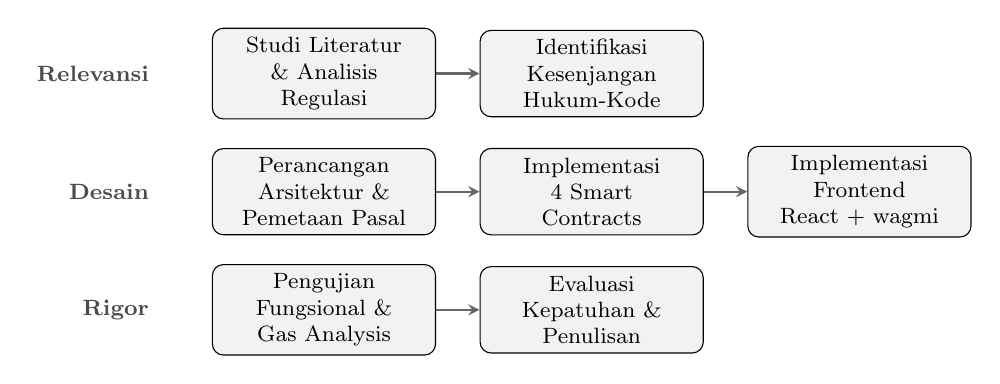
\begin{tikzpicture}[
 node distance=1.8cm,
 stage/.style={rectangle, draw, rounded corners=4pt, fill=black!5, minimum width=2.8cm, minimum height=0.7cm, text width=2.6cm, align=center, font=\footnotesize},
 arr/.style={->, >=stealth, thick, black!60},
 darr/.style={->, >=stealth, dashed, black!40, thick},
]
\node[rectangle, draw=none, font=\footnotesize\bfseries, text=black!70, anchor=east] at (-0.3,1.5) {Relevansi};
\node[stage] (s1) at (1.8,1.5) {Studi Literatur\\\& Analisis\\Regulasi};
\node[stage] (s2) at (5.2,1.5) {Identifikasi\\Kesenjangan\\Hukum-Kode};
\node[rectangle, draw=none, font=\footnotesize\bfseries, text=black!70, anchor=east] at (-0.3,0) {Desain};
\node[stage] (s3) at (1.8,0) {Perancangan\\Arsitektur \&\\Pemetaan Pasal};
\node[stage] (s4) at (5.2,0) {Implementasi\\4 Smart\\Contracts};
\node[stage] (s5) at (8.6,0) {Implementasi\\Frontend\\React + wagmi};
\node[rectangle, draw=none, font=\footnotesize\bfseries, text=black!70, anchor=east] at (-0.3,-1.5) {Rigor};
\node[stage] (s6) at (1.8,-1.5) {Pengujian\\Fungsional \&\\Gas Analysis};
\node[stage] (s7) at (5.2,-1.5) {Evaluasi\\Kepatuhan \&\\Penulisan};

% Horizontal
\draw[arr] (s1) -- (s2);
\draw[arr] (s3) -- (s4);
\draw[arr] (s4) -- (s5);
\draw[arr] (s6) -- (s7);

\end{tikzpicture}
\caption{Alur Penelitian dalam Tiga Siklus \textit{Design Science Research} (Hevner, 2007)}
\label{fig:alur-penelitian}
\end{figure}

Tahap 1: Studi Literatur dan Analisis Regulasi. Tahap ini mengidentifikasi permasalahan koperasi tradisional melalui studi terhadap UU 25/1992, PP 7/2021, dan Permenkop 8/2023, serta mengkaji literatur tentang blockchain untuk koperasi, tata kelola DAO, dan keamanan \textit{smart contract}. Analisis kesenjangan mengidentifikasi bahwa belum ada sistem yang memetakan ketentuan UU 25/1992 secara sistematis ke dalam \textit{smart contract}.

Tahap 2: Perancangan Arsitektur dan Smart Contract. Arsitektur sistem dirancang dengan empat \textit{smart contract} yang saling terintegrasi: LakomiToken (keanggotaan), LakomiVault (perbendaharaan dan SHU), LakomiGovern (tata kelola dan pemilihan), dan LakomiLoans (pinjaman). Setiap fungsi \textit{smart contract} dipetakan ke ketentuan spesifik UU 25/1992.

Tahap 3: Implementasi Smart Contract. \textit{Smart contract} diimplementasikan menggunakan Solidity 0.8.20 dengan Hardhat sebagai \textit{framework} pengembangan. Setiap kontrak menggunakan AccessControl dari OpenZeppelin untuk otorisasi berbasis peran dan ReentrancyGuard untuk perlindungan terhadap serangan \textit{reentrancy}.

Tahap 4: Implementasi Frontend. Aplikasi web dibangun menggunakan React 18 dengan TypeScript. Integrasi blockchain menggunakan wagmi v2 untuk koneksi \textit{wallet} dan interaksi dengan \textit{smart contract}. Antarmuka pengguna mencakup halaman \textit{dashboard} anggota, portal tata kelola, dan halaman kepatuhan regulasi.

Tahap 5: Pengujian Fungsional dan Gas Analysis. Pengujian dilakukan menggunakan Hardhat pada lingkungan DChain. Setiap ketentuan UU 25/1992 diverifikasi melalui skenario pengujian fungsional. Analisis gas dilakukan untuk mengukur biaya komputasi operasi utama koperasi.

Tahap 6: Evaluasi Kepatuhan dan Analisis Hasil. Hasil pengujian dievaluasi terhadap 26 ketentuan UU 25/1992. Analisis mencakup verifikasi kepatuhan fungsional, perbandingan dengan koperasi tradisional dan DAO berbasis token, serta pembahasan implikasi dan keterbatasan sistem.

\section{Arsitektur Sistem}

Lakomi dirancang dengan arsitektur tiga \textit{layer} yang memisahkan \textit{layer} keanggotaan, \textit{layer} kontrak, dan \textit{layer} blockchain. Diagram arsitektur sistem ditunjukkan pada Gambar~\ref{fig:arsitektur-3}.

\begin{figure}[H]
\centering
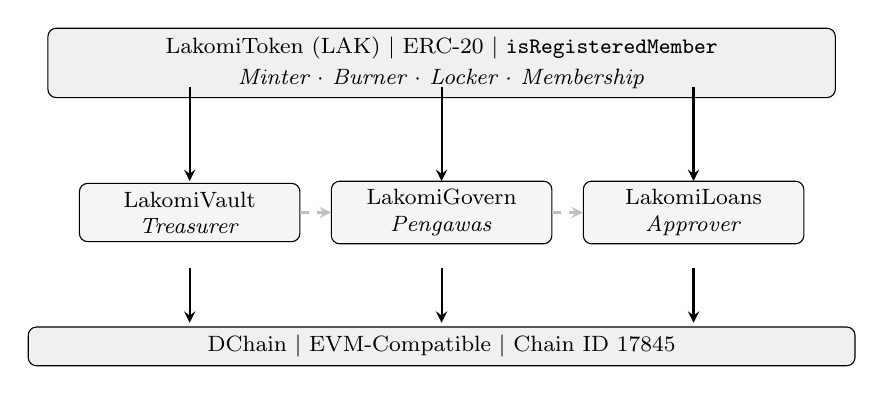
\begin{tikzpicture}[
 box/.style={rectangle, rounded corners=3pt, draw, minimum width=2.8cm, minimum height=0.45cm, font=\footnotesize, align=center, inner sep=3pt},
 arr/.style={->, >=stealth, thick},
 darr/.style={->, >=stealth, thick, dashed, gray!50},
]
\node[box, fill=black!6, minimum width=10cm] (token)
 at (0,2.5) {LakomiToken (LAK) $\mid$ ERC-20 $\mid$ \texttt{isRegisteredMember}\\[2pt]
 {\footnotesize\textit{Minter $\cdot$ Burner $\cdot$ Locker $\cdot$ Membership}}};
\draw[arr] (-3.2,2.2) -- (-3.2,1.0);
\draw[arr] (0,2.2) -- (0,1.0);
\draw[arr] (3.2,2.2) -- (3.2,1.0);
\node[box, fill=black!4] (vault) at (-3.2,0.6) {LakomiVault\\{\footnotesize\textit{Treasurer}}};
\node[box, fill=black!4] (govern) at (0,0.6)  {LakomiGovern\\{\footnotesize\textit{Pengawas}}};
\node[box, fill=black!4] (loans) at (3.2,0.6) {LakomiLoans\\{\footnotesize\textit{Approver}}};
\draw[darr] (vault.east) -- (govern.west);
\draw[darr] (govern.east) -- (loans.west);
\draw[arr] (-3.2,-0.1) -- (-3.2,-0.8);
\draw[arr] (0,-0.1) -- (0,-0.8);
\draw[arr] (3.2,-0.1) -- (3.2,-0.8);
\node[box, fill=black!6, minimum width=10.5cm]
 (chain) at (0,-1.1) {DChain $\mid$ EVM-Compatible $\mid$ Chain ID 17845};
\end{tikzpicture}
\caption{Arsitektur sistem Lakomi. LakomiToken berfungsi sebagai \textit{registry} keanggotaan. LakomiVault mengelola simpanan dan distribusi SHU. LakomiGovern menangani proposal, pemungutan suara, dan pemilihan. LakomiLoans menyediakan pinjaman dengan \textit{loan-to-value} berbasis kontribusi.}
\label{fig:arsitektur-3}
\end{figure}

Keempat \textit{smart contract} dan perannya dalam arsitektur adalah sebagai berikut:

\begin{enumerate}
	\item \textit{Membership Layer}, LakomiToken (LAK) berfungsi sebagai \textit{registry} keanggotaan berbasis ERC-20~\cite{eip20}. Setiap anggota yang terdaftar memiliki tepat satu suara dalam tata kelola, terlepas dari jumlah token yang dimiliki atau kontribusi simpanan. Kontrak ini mengelola empat peran: MINTER, BURNER, LOCKER, dan MEMBERSHIP.
	\item \textit{Contract Layer}, Tiga kontrak yang menangani fungsi inti koperasi:
	\begin{itemize}
		\item LakomiVault mengelola \textit{treasury} IDRX, tiga jenis simpanan (pokok, wajib, sukarela), dan distribusi SHU enam kategori sesuai Pasal 45(2).
		\item LakomiGovern menangani pembuatan proposal, pemungutan suara demokratis (satu-anggota-satu-suara), pemilihan pengurus, \textit{veto} pengawas, RAT tahunan, dan pembubaran koperasi.
		\item LakomiLoans menyediakan pinjaman mikro dengan \textit{loan-to-value} berbasis kontribusi, suku bunga tetap 5\% APY, dan jaminan 25\%.
	\end{itemize}
	\item \textit{Blockchain Layer}, Seluruh kontrak diterapkan pada DChain (EVM-compatible~\cite{wood2014ethereum}, Chain ID 17845), jaringan blockchain konsorsium pendidikan tinggi Indonesia.
\end{enumerate}

Lima peran mengatur sistem: PENGAWAS\_ROLE (pengawas dengan hak veto), APPROVER\_ROLE (persetujuan pinjaman), MEMBERSHIP\_ROLE (manajemen anggota), TREASURER\_ROLE (operasional \textit{vault}), dan GOVERN\_ROLE (distribusi SHU). Kontrak LakomiGovern memegang MEMBERSHIP\_ROLE pada token, memungkinkan pencabutan keanggotaan melalui tata kelola sesuai Pasal 31.

\section{Desain Smart Contract}

\subsection{Rasionalisasi Pemilihan Arsitektur}

Sebelum membahas detail implementasi, bagian ini menyajikan justifikasi desain untuk setiap keputusan arsitektural utama yang membedakan Lakomi dari pendekatan alternatif. Setiap keputusan dievaluasi terhadap tiga kriteria: kepatuhan terhadap UU 25/1992, keamanan teknis, dan kelayakan operasional.

Keputusan 1: Pemisahan Kontrak vs Monolitik. Arsitektur empat kontrak (Token, Vault, Govern, Loans) dipilih dibandingkan pendekatan monolitik (satu kontrak besar). Kepatuhan: setiap kontrak bertanggung jawab atas satu domain fungsional (keanggotaan, perbendaharaan, tata kelola, pinjaman), memudahkan verifikasi kepatuhan per pasal UU 25/1992 secara independen. Keamanan: \textit{blast radius} terbatas, jika satu kontrak mengalami kerentanan, kontrak lain tetap beroperasi, membatasi dampak serangan terhadap seluruh sistem. Kelayakan operasional: setiap kontrak dapat diperbarui secara independen tanpa memengaruhi kontrak lain, memungkinkan adaptasi bertahap terhadap perubahan regulasi; pengguna hanya membayar gas untuk kontrak yang relevan dengan transaksi mereka. Risiko kompleksitas interaksi antar-kontrak dimitigasi melalui \textit{wiring} yang ketat pada saat \textit{deployment} dan verifikasi dependensi melalui pengujian integrasi.

Keputusan 2: ERC-20 dengan Transfer Dinonaktifkan. LakomiToken mewarisi standar ERC-20 tetapi menonaktifkan fungsi transfer. Kepatuhan: sesuai Pasal 19(3) UU 25/1992, token keanggotaan bersifat \textit{intuitu personae} dan tidak dapat diperjualbelikan, sehingga mencegah spekulasi hak suara. Keamanan: dengan menonaktifkan transfer, token tidak dapat dicuri melalui \texttt{transferFrom()} atau disalahgunakan di pasar sekunder untuk memanipulasi tata kelola. Kelayakan operasional: dengan mewarisi ERC-20, token tetap kompatibel dengan \textit{wallet}, \textit{block explorer}, dan alat analitik yang mengharapkan antarmuka standar; jika regulasi berubah dan transfer diizinkan di masa depan, perubahan hanya memerlukan satu \textit{boolean flag} tanpa \textit{redeployment} atau migrasi data. Alternatif token kustom tanpa standar ditolak karena akan kehilangan interoperabilitas dengan ekosistem Ethereum.

Keputusan 3: RBAC 8-Peran vs Ownership Tunggal. Sistem menggunakan 8 peran terdistribusi dibandingkan model \texttt{Ownable} dengan satu pemilik. Kepatuhan: mencerminkan struktur organisasi koperasi (Pasal 21--39 UU 25/1992) yang memisahkan pengurus, pengawas, dan anggota, di mana setiap peran memiliki wewenang terbatas dan saling mengawasi. Keamanan: mitigasi \textit{single point of failure}, tidak ada satu akun yang memiliki kendali penuh, sehingga kompromi satu kunci privat tidak serta-merta membahayakan seluruh sistem; pemisahan antara pengusul, peninjau, dan pelaksana mencegah kolusi. Kelayakan operasional: setiap peran dapat diberikan kepada akun terpisah sesuai struktur organisasi koperasi riil, dan peran dapat dicabut atau dialihkan melalui mekanisme tata kelola tanpa \textit{redeployment} kontrak. Risiko kompleksitas manajemen peran dimitigasi melalui dokumentasi matriks akses pada Lampiran.

Keputusan 4: Suku Bunga Tetap vs Dinamis. Suku bunga pinjaman ditetapkan tetap 5\% APY dibandingkan model dinamis berbasis \textit{utilization rate}. Kepatuhan: Permenkop 8/2023 Pasal 43 mewajibkan prinsip kehati-hatian dalam pemberian pinjaman; suku bunga tetap rendah menjamin kepatuhan berkelanjutan dan melindungi anggota dari fluktuasi biaya. Keamanan: suku bunga tetap menghilangkan vektor serangan manipulasi pasar (\textit{oracle manipulation}) yang umum terjadi pada protokol DeFi dengan suku bunga dinamis. Kelayakan operasional: anggota dapat menghitung biaya pinjaman di muka tanpa bergantung pada kondisi pasar; suku bunga 5\% memastikan akses pinjaman bagi anggota dengan kapasitas finansial terbatas. Alternatif dinamis ditolak karena bertentangan dengan prinsip kesejahteraan anggota.

Keputusan 5: Kuorum 67\% vs Mayoritas Sederhana. Kuorum ditetapkan 67\% (dua per tiga) dibandingkan mayoritas sederhana (50\%+1). Kepatuhan: Pasal 24(2) UU 25/1992 mengamanatkan keputusan berdasarkan suara terbanyak; Lakomi menetapkan ambang dua per tiga sebagai interpretasi dukungan mayoritas yang memastikan legitimasi setara semangat musyawarah koperasi. Keamanan: kuorum tinggi melindungi dari serangan \textit{governance takeover} di mana penyerang mendaftarkan anggota palsu untuk meloloskan proposal berbahaya, dibutuhkan 67\% dari total anggota, bukan hanya 50\%+1. Kelayakan operasional: perlindungan minoritas, anggota minoritas hingga 33\% tidak dapat diabaikan sepenuhnya, mendorong musyawarah dan kompromi; mekanisme \textit{abstain} dihitung sebagai partisipasi tanpa memihak, membantu pencapaian kuorum. Risiko kebuntuan dimitigasi melalui penghitungan suara \textit{abstain} sebagai kontribusi kuorum.

Keputusan 6: Agunan 25\% vs Overcollateralization. Agunan ditetapkan 25\% dari pokok pinjaman dibandingkan model \textit{overcollateralization} 150\% pada protokol DeFi. Kepatuhan: Permenkop 8/2023 Pasal 43--45 mengatur BMPP dan prinsip kehati-hatian; agunan 25\% memberikan perlindungan terhadap gagal bayar tanpa membebani anggota secara berlebihan, sesuai prinsip kesejahteraan anggota. Keamanan: agunan dalam token LAK dikunci secara on-chain melalui LOCKER\_ROLE, tidak dapat dilepaskan sepihak oleh peminjam; \textit{markDefaulted()} dan \texttt{claimCollateral()} memungkinkan pemulihan kerugian secara terprogram. Kelayakan operasional: agunan rendah (25\%) memungkinkan akses pinjaman bagi anggota bermodal kecil yang tidak mampu memenuhi \textit{overcollateralization} 150\%; dikombinasikan dengan LTV bertingkat (30\%/50\%/70\%), sistem memberikan insentif bagi anggota untuk meningkatkan kontribusi simpanan tanpa menghalangi akses pinjaman dasar.

\begin{table}[H]
\centering
\caption{Justifikasi Keputusan Desain Arsitektural}
\label{tab:design-decisions}
\small
\begin{tabular}{p{0.18\textwidth}p{0.13\textwidth}p{0.28\textwidth}p{0.31\textwidth}}
\toprule
\textbf{Keputusan} & \textbf{Pilihan} & \textbf{Alternatif (Ditolak)} & \textbf{Alasan Penolakan} \\
\midrule
Arsitektur Kontrak & 4 kontrak terpisah & 1 kontrak monolitik & \textit{Blast radius} besar, sulit diverifikasi per pasal \\
Model Token & ERC-20 non-transferable & Token kustom tanpa standar & Kehilangan interoperabilitas ekosistem \\
Model Akses & RBAC 8-peran & \texttt{Ownable} tunggal & \textit{Single point of failure}, tidak sesuai UU \\
Suku Bunga & Tetap 5\% APY & Dinamis (\textit{utilization rate}) & Tidak ada kepastian biaya, bertentangan dengan prinsip koperasi \\
Kuorum & 67\% (dua per tiga) & 50\%+1 (mayoritas sederhana) & Rentan manipulasi, legitimasi rendah \\
Agunan & 25\% tetap & 150\% (\textit{overcollateralized}) & Mengecualikan anggota bermodal kecil \\
\bottomrule
\end{tabular}
\end{table}

\subsection{Struktur Data}

Setiap \textit{smart contract} mendefinisikan struktur data yang memetakan ketentuan UU 25/1992:

\begin{enumerate}
	\item LakomiToken, \texttt{isRegisteredMember} (\textit{mapping} boolean) memisahkan identitas keanggotaan dari kepemilikan token. \texttt{MAX\_SUPPLY} ditetapkan 1.000.000 LAK (18 desimal) dengan alokasi \textit{default} 100 LAK per anggota baru. Transfer token dinonaktifkan (\texttt{transfersEnabled = false}) sesuai Pasal 19(3).
	\item LakomiVault, \texttt{simpananPokok}, \texttt{simpananWajib}, dan \texttt{shares} (\textit{balance} sukarela) melacak tiga jenis simpanan sesuai Pasal 41(2) dan Permenkop 8/2023. \texttt{accumulatedRevenue} mengakumulasi pendapatan bunga pinjaman. \texttt{danaCadangan} melacak dana cadangan sesuai Pasal 41(2)(c) dan 45(3).
	\item LakomiGovern, \texttt{proposals} (\textit{mapping} ke struct Proposal) menyimpan proposal lengkap dengan status, suara, dan \textit{timelock}. \texttt{elections} (\textit{nested mapping}) melacak kandidat, suara, dan masa jabatan untuk setiap peran. \texttt{quorumNumerator} (default 67) menetapkan ambang kuorum dua per tiga.
	\item LakomiLoans, \texttt{loans} (\textit{mapping} ke struct Loan) melacak pinjaman dengan status, pokok, bunga, agunan, dan riwayat pembayaran. \texttt{contributionTier} berbasis \texttt{cumulativeSimpanan} menentukan \textit{loan-to-value} (30\%, 50\%, 70\%).
\end{enumerate}

\subsection{Kontrol Akses Berbasis Peran}

Sistem menerapkan \textit{Role-Based Access Control} (RBAC) menggunakan AccessControl dari OpenZeppelin. Delapan peran didefinisikan di seluruh kontrak:

\begin{enumerate}
	\item DEFAULT\_ADMIN\_ROLE, Administrator sistem yang mengelola peran lainnya.
	\item MEMBERSHIP\_ROLE, Mengelola pendaftaran dan pencabutan keanggotaan.
	\item MINTER\_ROLE, Mencetak token LAK baru pada pendaftaran anggota.
	\item BURNER\_ROLE, Membakar token pada pencabutan keanggotaan.
	\item LOCKER\_ROLE, Mengunci token sebagai agunan pinjaman.
	\item TREASURER\_ROLE, Mengelola operasional \textit{vault} dan simpanan.
	\item PENGAWAS\_ROLE, Melakukan veto proposal dan audit keuangan (Pasal 38--39).
	\item APPROVER\_ROLE, Menyetujui permohonan pinjaman.
\end{enumerate}

Setiap fungsi \textit{state-modifying} dilindungi oleh \texttt{onlyRole} atau \texttt{onlyRegisteredMember}. Fungsi pembacaan data bersifat publik.

\subsection{Fungsi Utama per Ketentuan UU 25/1992}

Tabel~\ref{tab:fungsi-uu} merangkum fungsi utama setiap kontrak yang memetakan ketentuan spesifik UU 25/1992. Pemetaan ini mencakup 13 fungsi yang tersebar di empat kontrak, masing-masing mengimplementasikan satu atau lebih pasal dari UU 25/1992 dan peraturan turunannya. Setiap fungsi dirancang untuk memenuhi kondisi persyaratan (prasyarat), aksi (operasi yang dijalankan), kendala (batasan), dan aktor berwenang (pihak yang memiliki otorisasi) yang diturunkan langsung dari teks hukum. Tabel ini berfungsi sebagai acuan utama untuk memverifikasi bahwa setiap ketentuan UU 25/1992 memiliki representasi yang dapat dieksekusi dalam kode.

\begin{table}[H]
\centering
\caption{Pemetaan Fungsi Smart Contract ke Ketentuan UU 25/1992}
\label{tab:fungsi-uu}
\footnotesize
\resizebox{\textwidth}{!}{\begin{tabular}{p{0.15\textwidth}p{0.14\textwidth}p{0.40\textwidth}p{0.25\textwidth}}
\toprule
\textbf{Kontrak} & \textbf{Pasal} & \textbf{Fungsi} & \textbf{Deskripsi} \\
\midrule
\multirow{4}{*}{LakomiToken} & 5(1), 17--18 & \texttt{registerMember()} & Pendaftaran anggota mandiri \\
 & 19(3) & \texttt{transfersEnabled = false} & Token tidak dapat dipindahtangankan \\
 & 19--21 & \texttt{resignMembership()} & Pengunduran diri sukarela \\
 & 19(2), 30(2)(b) & \texttt{revokeMembership()} & Pencabutan melalui tata kelola \\
\midrule
\multirow{3}{*}{LakomiVault} & 41(2) & \texttt{paySimpananPokok/Wajib()} & Pembayaran simpanan \\
 & 41(2)(c), 45(2-3) & \texttt{danaCadangan} & Pelacakan dana cadangan \\
 & 45(1--2) & \texttt{distributeSHU()} & Distribusi SHU 6 kategori \\
\midrule
\multirow{4}{*}{LakomiGovern} & 24(3) & \texttt{getVotingPower() $\to$ 1} & Satu suara per anggota \\
 & 24(2) \& desain & \texttt{quorumNumerator = 67} & Kuorum dua per tiga \\
 & 26--27 & \texttt{scheduleAnnualRAT()} & RAT tahunan \\
 & 29--30 & \texttt{beginElection() $\to$ finalizeElection()} & Pemilihan pengurus \\
\midrule
\multirow{2}{*}{LakomiLoans} & 41(2)(a), 44 & \texttt{requestLoan()} & Pinjaman LTV berbasis kontribusi \\
 & Permenkop 8/2023 Ps 43--45 & \texttt{tieredLTV + 5\% APY} & Batas pinjaman dan suku bunga \\
\bottomrule
\end{tabular}}
\end{table}

\subsection{Event Logging}

Setiap \textit{smart contract} mendefinisikan \textit{event} yang memfasilitasi pelacakan aktivitas on-chain dan membangun \textit{audit trail} yang lengkap. \textit{Event-event} ini dapat dimonitor melalui \textit{block explorer} DChain untuk keperluan audit dan verifikasi eksternal:

\begin{itemize}
	\item \texttt{MemberRegistered(address member)}, Dipancarkan oleh LakomiToken ketika anggota baru berhasil mendaftar.
	\item \texttt{MemberResigned(address member)}, Dipancarkan ketika anggota mengundurkan diri secara sukarela.
	\item \texttt{SimpananPaid(address member, uint256 amount, string simpananType)}, Dipancarkan oleh LakomiVault pada setiap pembayaran simpanan (pokok, wajib, sukarela).
	\item \texttt{SHUDistributed(uint256 distributionsId, uint256 totalAmount)}, Dipancarkan ketika distribusi SHU enam kategori berhasil dieksekusi.
	\item \texttt{ProposalCreated(uint256 proposalId, address proposer)}, Dipancarkan oleh LakomiGovern pada pembuatan proposal baru.
	\item \texttt{VoteCast(uint256 proposalId, address voter, uint8 vote)}, Dipancarkan pada setiap pemungutan suara.
	\item \texttt{ElectionFinalized(bytes32 role, address winner)}, Dipancarkan ketika pemilihan pengurus selesai dan pemenang ditetapkan.
	\item \texttt{LoanRequested(uint256 loanId, address borrower, uint256 amount)}, Dipancarkan oleh LakomiLoans pada pengajuan pinjaman.
	\item \texttt{LoanRepaid(uint256 loanId, uint256 amount)}, Dipancarkan ketika pinjaman dilunasi.
\end{itemize}

\subsection{Justifikasi Parameter Sistem}

Setiap parameter dalam sistem ditetapkan berdasarkan pertimbangan regulasi dan praktis. Tabel~\ref{tab:parameter} merangkum justifikasi untuk setiap parameter utama.

\begin{table}[H]
\centering
\caption{Justifikasi Parameter Sistem}
\label{tab:parameter}
\footnotesize
\begin{tabular}{p{0.18\textwidth}p{0.12\textwidth}p{0.62\textwidth}}
\toprule
\textbf{Parameter} & \textbf{Nilai} & \textbf{Justifikasi} \\
\midrule
Kuorum & 67\% & Mencerminkan prinsip koperasi bahwa keputusan memerlukan konsensus mayoritas signifikan. Pasal 24(2) UU 25/1992 mengamanatkan keputusan berdasarkan suara terbanyak; Lakomi menetapkan nilai dua per tiga sebagai interpretasi dukungan mayoritas yang memastikan legitimasi keputusan. \\
\addlinespace
Periode Voting & 7 hari & Memberikan waktu yang memadai bagi anggota untuk meninjau proposal tanpa memperlambat operasional koperasi. \\
\addlinespace
Timelock Eksekusi & 24 jam & Memberikan jendela pengamanan bagi pengawas untuk melakukan veto sebelum proposal dieksekusi (Pasal 38). \\
\addlinespace
Suku Bunga & 5\% APY & Lebih rendah dari suku bunga komersial, sesuai prinsip koperasi yang mengutamakan kesejahteraan anggota. Permenkop 8/2023 Pasal 43 mewajibkan prinsip kehati-hatian dalam pemberian pinjaman. \\
\addlinespace
Agunan & 25\% & Memberikan perlindungan terhadap risiko gagal bayar tanpa membebani anggota secara berlebihan. \\
\addlinespace
Auto-approval & $\leq$ 200 IDRX & Memungkinkan akses cepat ke dana darurat untuk pinjaman kecil tanpa menunggu proses tata kelola. \\
\addlinespace
LTV Tier 1/2/3 & 30\%/50\%/70\% & Memberikan insentif bagi anggota untuk meningkatkan kontribusi simpanan, semakin besar kontribusi, semakin besar kapasitas pinjaman, tanpa memengaruhi hak suara. \\
\bottomrule
\end{tabular}
\end{table}

Parameter-parameter dalam Tabel~\ref{tab:parameter} membentuk kerangka operasional koperasi yang mencerminkan keseimbangan antara efisiensi, keamanan, dan kepatuhan regulasi. Kuorum 67\% dan periode voting 7 hari memastikan bahwa keputusan tata kelola memiliki legitimasi demokratis yang kuat, setiap anggota memiliki waktu yang cukup untuk meninjau proposal dan memberikan suara, sementara ambang dua per tiga mencegah keputusan diambil oleh minoritas kecil. Timelock 24 jam memberikan jendela keamanan yang memungkinkan pengawas melakukan intervensi terhadap proposal yang berpotensi merugikan, mencerminkan mekanisme \textit{checks and balances} yang diamanatkan Pasal 38. Suku bunga 5\% APY menyeimbangkan keberlanjutan operasional koperasi dengan prinsip kesejahteraan anggota, cukup rendah untuk tidak membebani peminjam, namun cukup untuk menghasilkan pendapatan yang mendanai operasional dan distribusi SHU. Agunan 25\% dipilih sebagai titik tengah antara perlindungan terhadap gagal bayar dan aksesibilitas pinjaman, terlalu tinggi akan mengecualikan anggota dengan kontribusi terbatas, terlalu rendah akan meningkatkan risiko bagi \textit{vault}. Auto-approval untuk pinjaman kecil ($\leq$ 200 IDRX) mengakui bahwa pinjaman darurat memerlukan respons cepat, sementara mekanisme LTV bertingkat (30\%/50\%/70\%) menciptakan insentif positif: anggota yang berkontribusi lebih besar melalui simpanan mendapatkan kapasitas pinjaman yang lebih besar, namun hak suara mereka tetap setara dengan anggota lainnya.

LakomiGovern mengimplementasikan model tata kelola demokratis di mana setiap anggota terdaftar memegang tepat satu suara. Siklus hidup proposal diilustrasikan pada Gambar~\ref{fig:proposal-lifecycle}. Proposal dimulai dari status Created ketika anggota menginisiasi pengajuan, kemudian memasuki masa Active selama 7 hari di mana anggota memberikan suara. Setelah periode voting berakhir, proposal yang memenuhi kuorum 67\% dan memiliki suara For lebih banyak dari Against akan berstatus Succeeded dan masuk ke antrean eksekusi.

\begin{figure}[H]
\centering
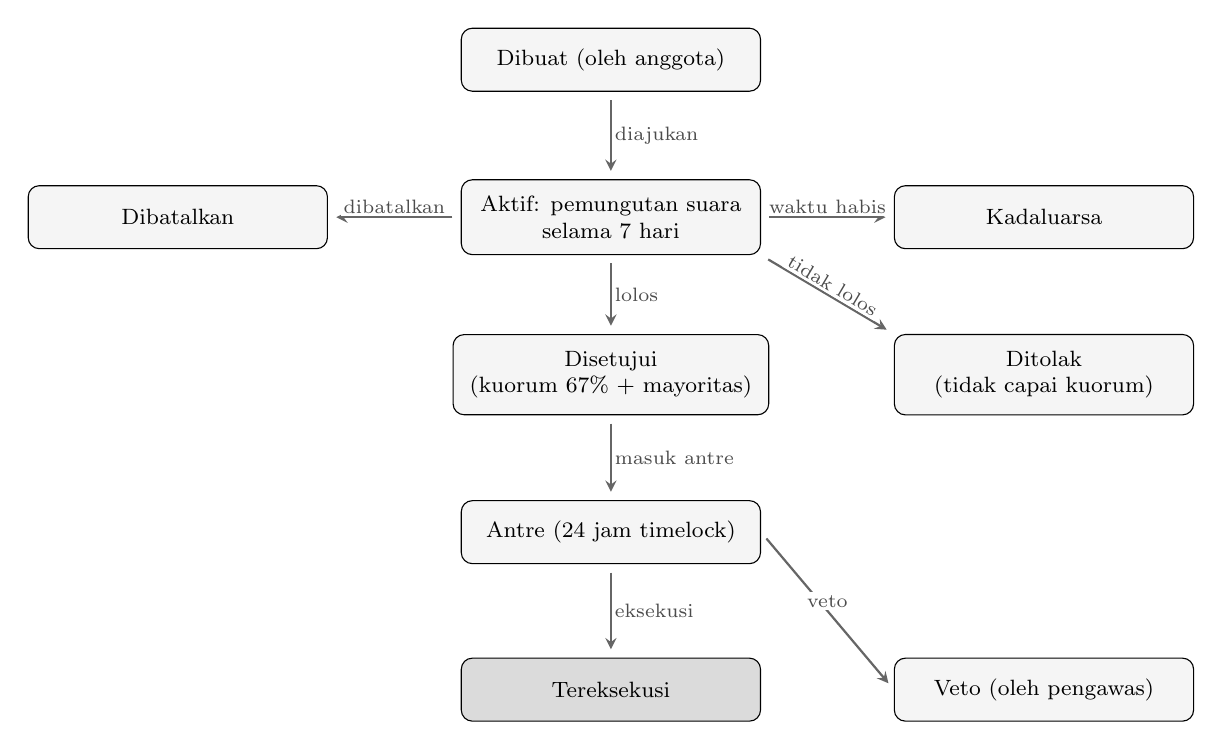
\begin{tikzpicture}[
 box/.style={rectangle, draw, rounded corners=4pt, minimum width=3.8cm, minimum height=0.8cm, font=\footnotesize, align=center, inner sep=6pt, fill=black!4},
 endbox/.style={box, fill=black!14},
 arr/.style={->, >=stealth, thick, black!60, shorten >=3pt, shorten <=3pt},
 lbl/.style={font=\scriptsize, fill=white, inner sep=1pt, text=black!70},
]
\node[box] (create) at (0,9.0) {Dibuat (oleh anggota)};
\node[box] (voting) at (0,7.0) {Aktif: pemungutan suara\\selama 7 hari};
\node[box] (timeout) at (5.5,7.0) {Kadaluarsa};
\node[box] (cancel) at (-5.5,7.0) {Dibatalkan};
\node[box] (def) at (5.5,5.0) {Ditolak\\(tidak capai kuorum)};
\node[box] (succ) at (0,5.0) {Disetujui\\(kuorum 67\% + mayoritas)};
\node[box] (queue) at (0,3.0) {Antre (24 jam timelock)};
\node[box] (vetoed) at (5.5,1.0) {Veto (oleh pengawas)};
\node[endbox] (exec) at (0,1.0) {Tereksekusi};

\draw[arr] (create) -- (voting) node[lbl, midway, right] {diajukan};
\draw[arr] (voting.west) -- (cancel.east) node[lbl, midway, above] {dibatalkan};
\draw[arr] (voting.east) -- (timeout.west) node[lbl, midway, above] {waktu habis};
\draw[arr] (voting) -- (succ) node[lbl, midway, right] {lolos};
\draw[arr] (voting.south east) -- (def.north west) node[lbl, midway, above, sloped] {tidak lolos};
\draw[arr] (succ) -- (queue) node[lbl, midway, right] {masuk antre};
\draw[arr] (queue) -- (exec) node[lbl, midway, right] {eksekusi};
\draw[arr] (queue.east) -- (vetoed.west) node[lbl, midway, above] {veto};
\end{tikzpicture}
\caption{Siklus Hidup Proposal pada LakomiGovern}
\label{fig:proposal-lifecycle}
\end{figure}

Proposal melalui empat tahap: (1) pembuatan oleh anggota terdaftar, (2) pemungutan suara selama 7 hari, (3) verifikasi kuorum 67\%, dan (4) eksekusi setelah \textit{timelock} 24 jam. Proposal yang tidak mencapai kuorum dinyatakan Ditolak, sementara yang melebihi batas waktu dinyatakan Kadaluarsa. Pemegang PENGAWAS\_ROLE dapat mem-veto proposal yang telah masuk antre sebelum eksekusi. Pengusul proposal juga dapat membatalkan proposalnya sendiri selama masih dalam masa Aktif.

Untuk pemilihan pengurus (Pasal 29--30), setiap anggota dapat mendaftar sebagai kandidat. Anggota memberikan satu suara per pemilihan, dan kandidat dengan suara terbanyak menang. Peran diberikan secara otomatis dengan masa jabatan 365 hari.

Distribusi SHU diawali dengan menghitung SHU yang dapat didistribusikan. Sebesar 10\% dari total pendapatan (\texttt{accumulatedRevenue}) disisihkan sebagai cadangan operasional sebelum distribusi:

\begin{equation}
\text{SHU}_{\text{distributable}} = \text{Revenue} - \text{Cadangan}_{\text{operasional}}(10\%)
\label{eq:shu-dist}
\end{equation}

\noindent dengan \textit{Revenue} merupakan total pendapatan yang terakumulasi dari bunga pinjaman anggota dan sumber pendapatan koperasi lainnya, sedangkan cadangan operasional sebesar 10\% digunakan untuk membiayai operasional sistem dan antisipasi risiko.

SHU yang dapat didistribusikan kemudian dialokasikan ke enam kategori sesuai ketentuan Pasal 45(2) UU 25/1992 dengan proporsi sebagai berikut:

\begin{equation}
\begin{aligned}
\text{Dana Cadangan} &= \text{SHU}_{\text{dist}} \times 5\% \\
\text{Jasa Modal} &= \text{SHU}_{\text{dist}} \times 40\% \quad \text{(pro-rata berdasarkan \textit{shares})} \\
\text{Jasa Usaha} &= \text{SHU}_{\text{dist}} \times 40\% \quad \text{(pro-rata berdasarkan \textit{shares})} \\
\text{Dana Pendidikan} &= \text{SHU}_{\text{dist}} \times 5\% \\
\text{Dana Pengurus} &= \text{SHU}_{\text{dist}} \times 5\% \\
\text{Dana Kesejahteraan Sosial} &= \text{SHU}_{\text{dist}} \times 5\%
\end{aligned}
\label{eq:shu-split}
\end{equation}

Alokasi Jasa Modal dan Jasa Usaha masing-masing sebesar 40\% mencerminkan kontribusi ganda anggota, sebagai penyetor modal melalui simpanan dan sebagai pengguna jasa koperasi melalui pinjaman, sesuai dengan prinsip keanggotaan ganda yang dianut UU 25/1992. Kedua komponen ini didistribusikan secara pro-rata berdasarkan \textit{shares} masing-masing anggota. Proporsi ini ditetapkan sebagai nilai \textit{basis points} yang dapat dikonfigurasi melalui mekanisme tata kelola, memungkinkan setiap koperasi untuk menyesuaikan alokasi SHU tanpa melakukan \textit{redeployment} kontrak.

Bunga pinjaman dihitung menggunakan formula sederhana tahunan:

\begin{equation}
\text{Bunga} = \frac{P \times 5\% \times D}{365}
\label{eq:bunga}
\end{equation}

\noindent dengan $P$ adalah pokok pinjaman dalam IDRX dan $D$ adalah durasi pinjaman dalam hari. Suku bunga 5\% APY (\textit{Annual Percentage Yield}) ditetapkan sebagai suku bunga tetap yang lebih rendah dibandingkan suku bunga pinjaman komersial, sesuai prinsip kehati-hatian yang diwajibkan Permenkop 8/2023 Pasal 43~\cite{permenkop82023}. Formula ini memastikan bahwa perhitungan bunga bersifat proporsional terhadap durasi, semakin singkat periode pinjaman, semakin kecil bunga yang dibebankan, sehingga memberikan insentif bagi anggota untuk melunasi pinjaman tepat waktu.

\section{Perancangan Keamanan}

Sistem Lakomi mengimplementasikan empat lapisan keamanan yang terintegrasi untuk melindungi aset dan memastikan integritas tata kelola koperasi.

\subsection{Kontrol Akses Berbasis Peran}

Seluruh fungsi \textit{state-modifying} pada keempat kontrak dilindungi oleh mekanisme \texttt{onlyRole} dari OpenZeppelin AccessControl. Delapan peran didistribusikan ke akun yang berbeda, memastikan bahwa tidak ada satu entitas pun yang memiliki kendali penuh atas sistem. Pemisahan peran ini mencegah skenario di mana administrator tunggal dapat menyetujui pinjaman kepada dirinya sendiri atau mendistribusikan SHU secara sepihak.

\subsection{Perlindungan Reentrancy}

Setiap fungsi yang melibatkan transfer dana, termasuk \texttt{disburse()} pada LakomiLoans, \texttt{distributeSHU()} pada LakomiVault, dan \texttt{claimSHU()}, dilindungi oleh \texttt{nonReentrant} modifier dari OpenZeppelin ReentrancyGuard. Mekanisme ini mencegah serangan \textit{reentrancy} di mana penyerang dapat memanggil fungsi secara rekursif sebelum \textit{state} diperbarui, yang berpotensi menguras dana \textit{vault}.

\subsection{Veto Pengawas sebagai Circuit Breaker}

PENGAWAS\_ROLE memiliki kemampuan untuk mem-veto proposal yang telah lolos pemungutan suara sebelum eksekusi. Mekanisme ini berfungsi sebagai \textit{circuit breaker} terhadap proposal berbahaya yang mungkin lolos karena manipulasi suara atau ketidaktahuan anggota. Veto hanya dapat dilakukan oleh pemegang peran pengawas (bukan oleh anggota biasa atau pengurus), mencerminkan pemisahan kekuasaan antara eksekutif (pengurus) dan pengawas sebagaimana diamanatkan dalam Pasal 38--39 UU 25/1992.

\subsection{Non-Transferabilitas Token Keanggotaan}

Token LAK bersifat tidak dapat dipindahtangankan (\texttt{transfersEnabled = false}). Keputusan desain ini memastikan bahwa keanggotaan koperasi tidak dapat diperjualbelikan di pasar sekunder, mencegah spekulasi hak suara, dan mematuhi prinsip \textit{intuitu personae} dalam keanggotaan koperasi sebagaimana diatur dalam Pasal 19(3) UU 25/1992.

\section{Desain Frontend}

\subsection{Arsitektur Aplikasi}

\textit{Frontend} dibangun menggunakan React 18 dengan TypeScript untuk menjamin \textit{type safety} pada interaksi dengan \textit{smart contract}. Integrasi blockchain menggunakan library wagmi v2 yang menyediakan \textit{React Hooks} untuk koneksi \textit{wallet}, pembacaan \textit{state} on-chain, dan pengiriman transaksi. Pengguna menghubungkan \textit{wallet} MetaMask ke jaringan DChain (Chain ID 17845) untuk berinteraksi dengan sistem.

Komunikasi dengan \textit{smart contract} dilakukan melalui \textit{provider} JSON-RPC DChain. Untuk operasi baca (\textit{read-only}), \textit{frontend} menggunakan \texttt{useContractRead} yang tidak memerlukan konfirmasi pengguna. Untuk operasi tulis (\textit{state-modifying}), \textit{frontend} menggunakan \texttt{useContractWrite} yang memicu \textit{pop-up} MetaMask untuk persetujuan transaksi oleh pengguna.

\subsection{Halaman dan Fungsionalitas}

Sistem menyediakan empat halaman utama yang dirancang sesuai dengan peran pengguna:

\begin{enumerate}
	\item \textit{Dashboard} Anggota, Halaman utama yang menampilkan status keanggotaan (\texttt{isRegisteredMember}), saldo simpanan pokok, simpanan wajib, dan simpanan sukarela, serta \textit{tier} kontribusi terkini. Anggota dapat melakukan pembayaran simpanan pokok (100 IDRX, satu kali), simpanan wajib (10 IDRX per 30 hari), dan simpanan sukarela (jumlah bebas) melalui formulir yang terhubung langsung ke LakomiVault. Halaman ini juga menampilkan riwayat transaksi simpanan dan klaim SHU.
	
	\item Portal Tata Kelola, Menyediakan antarmuka lengkap untuk partisipasi dalam tata kelola koperasi. Anggota dapat membuat proposal baru dengan memilih tipe proposal (SPEND, PARAMETER, MEMBERSHIP, RAT\_ANNUAL, CUSTOM) dan memberikan deskripsi. Halaman ini menampilkan daftar proposal aktif beserta status, jumlah suara, dan waktu tersisa. Anggota memberikan suara (For, Against, Abstain) melalui tombol yang terhubung ke fungsi \texttt{castVote()}. Portal ini juga menampilkan status RAT tahunan dan informasi pemilihan pengurus, termasuk daftar kandidat dan hasil pemilihan.
	
	\item Portal Pinjaman, Memungkinkan anggota mengajukan pinjaman dengan menentukan jumlah (dalam IDRX) dan durasi (dalam hari). Sistem secara otomatis menghitung \textit{loan-to-value} maksimum berdasarkan \textit{tier} kontribusi anggota dan menampilkan jumlah pinjaman yang tersedia. Anggota dapat melihat status permohonan pinjaman (Pending, Approved, Active, Repaid), melakukan pembayaran cicilan, dan melunasi pinjaman. Agunan dalam token LAK ditampilkan secara transparan.
	
	\item Halaman Kepatuhan Regulasi, Menampilkan seluruh 26 ketentuan UU 25/1992 yang telah diimplementasikan dalam sistem. Setiap ketentuan ditampilkan sebagai kartu (\textit{card}) yang berisi: nomor dan teks pasal, fungsi \textit{smart contract} yang mengimplementasikannya, bukti implementasi berupa nama fungsi dan parameter, serta status verifikasi. Ketentuan dikelompokkan berdasarkan kategori: Anggota, Simpanan, Pinjaman, dan Tata Kelola. Halaman ini berfungsi sebagai bukti \textit{on-chain compliance} yang dapat diverifikasi secara publik.
\end{enumerate}

\section{Alur Kerja Sistem}

Bagian ini menjelaskan alur kerja sistem untuk tiga skenario penggunaan utama.

\subsection{Skenario 1: Pendaftaran Anggota dan Simpanan}

\begin{figure}[H]
\centering
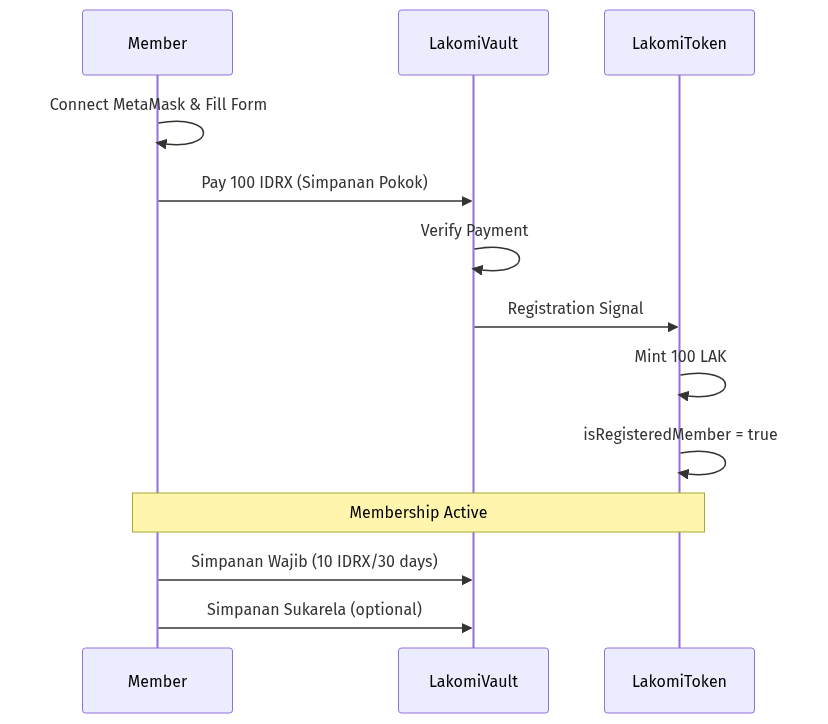
\includegraphics[width=0.75\textwidth]{figures/swimlane-daftar.png}
\caption{Diagram Alir Skenario 1: Pendaftaran Anggota dan Simpanan}
\label{fig:swimlane-1}
\end{figure}

\begin{enumerate}
	\item Calon anggota membuka aplikasi dan menghubungkan \textit{wallet} MetaMask ke jaringan DChain.
	\item Calon anggota mengisi formulir pendaftaran dan melakukan pembayaran simpanan pokok (100 IDRX) melalui \textit{smart contract} LakomiVault.
	\item LakomiVault memverifikasi pembayaran dan memberi sinyal ke LakomiToken.
	\item LakomiToken mencetak 100 LAK dan menetapkan \texttt{isRegisteredMember = true}.
	\item Anggota dapat melakukan pembayaran simpanan wajib (10 IDRX per 30 hari) dan simpanan sukarela kapan saja.
\end{enumerate}

\subsection{Skenario 2: Tata Kelola dan Pemungutan Suara}

\begin{figure}[H]
\centering
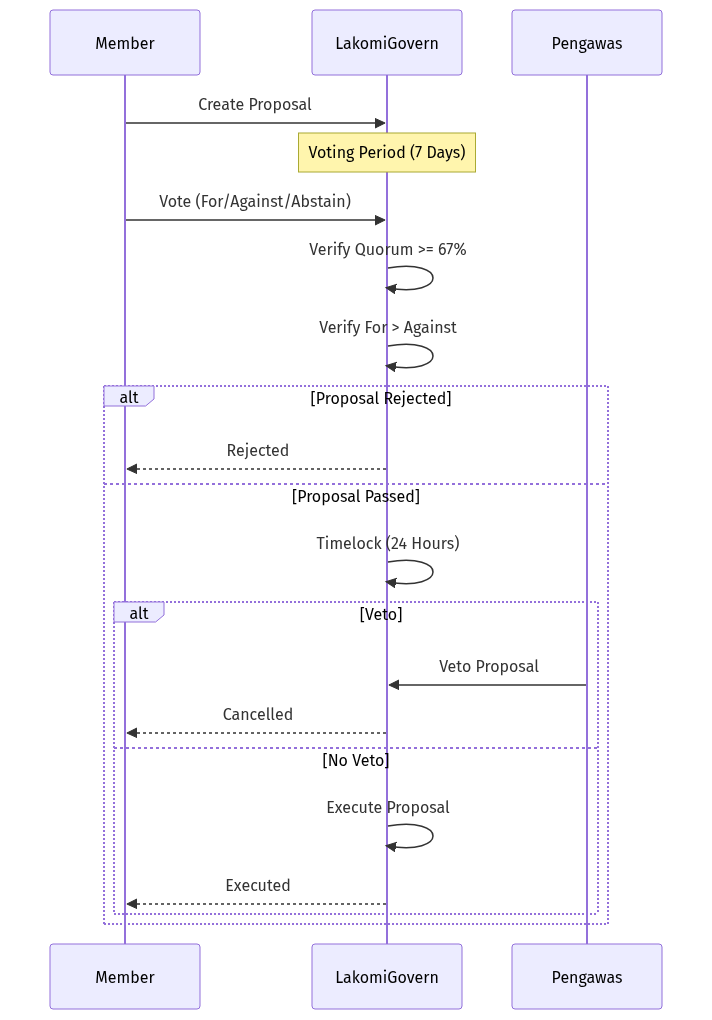
\includegraphics[width=0.75\textwidth]{figures/swimlane-tatakelola.png}
\caption{Diagram Alir Skenario 2: Tata Kelola dan Pemungutan Suara}
\label{fig:swimlane-2}
\end{figure}

\begin{enumerate}
	\item Anggota terdaftar membuat proposal melalui LakomiGovern dengan menentukan tipe (SPEND, PARAMETER, MEMBERSHIP, RAT\_ANNUAL, CUSTOM).
	\item Proposal memasuki masa pemungutan suara 7 hari. Setiap anggota memberikan satu suara (For, Against, atau Abstain).
	\item Setelah periode berakhir, sistem memverifikasi kuorum: $\text{totalVotes} \geq \text{memberCount} \times 67\%$ dan $\text{forVotes} > \text{againstVotes}$.
	\item Proposal yang lolos memasuki \textit{timelock} 24 jam sebelum dapat dieksekusi.
	\item Pemegang PENGAWAS\_ROLE dapat mem-veto proposal sebelum eksekusi sesuai Pasal 38.
\end{enumerate}

\subsection{Skenario 3: Pengajuan dan Pelunasan Pinjaman}

\begin{figure}[H]
\centering
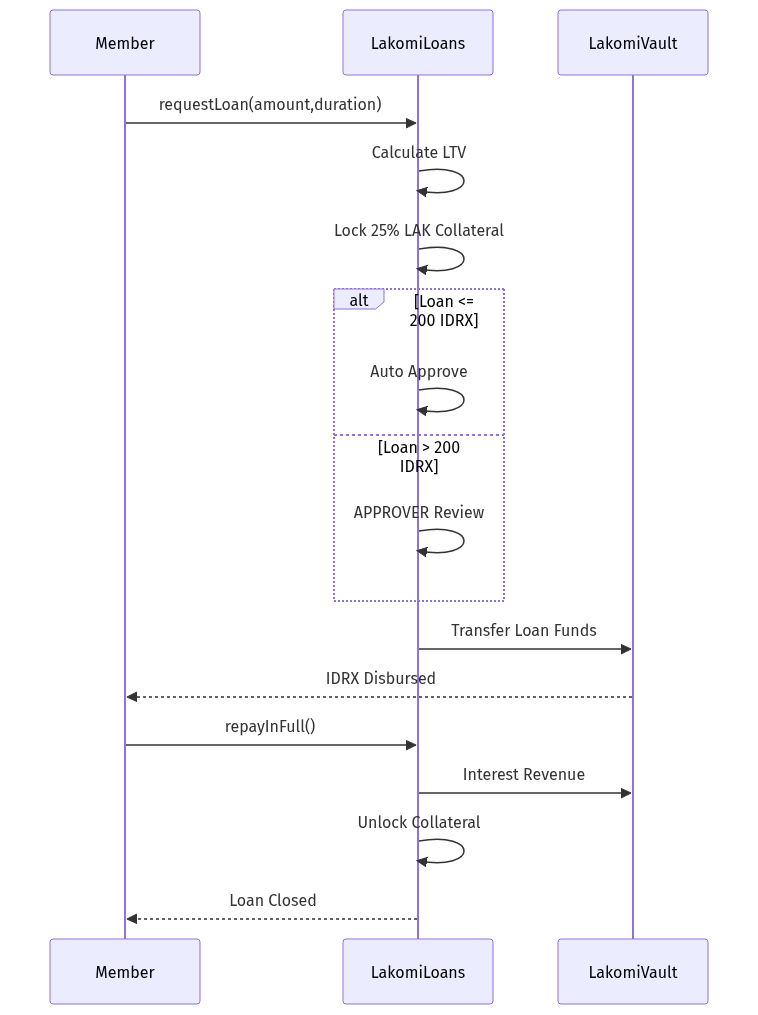
\includegraphics[width=0.75\textwidth]{figures/swimlane-pinjaman.png}
\caption{Diagram Alir Skenario 3: Pengajuan dan Pelunasan Pinjaman}
\label{fig:swimlane-3}
\end{figure}

\begin{enumerate}
	\item Anggota mengajukan pinjaman melalui \texttt{requestLoan()} dengan menentukan jumlah dan durasi.
	\item LakomiLoans menghitung \textit{loan-to-value} berdasarkan \textit{tier} kontribusi: $\text{maxLoan} = \text{contribution} \times \text{LTV} / 10000$.
	\item Agunan sebesar 25\% dari pokok pinjaman dalam token LAK dikunci oleh LOCKER\_ROLE.
	\item Pinjaman di bawah 200 IDRX disetujui otomatis; pinjaman lebih besar memerlukan persetujuan APPROVER\_ROLE.
	\item Dana IDRX ditransfer dari LakomiVault ke peminjam.
	\item Peminjam melunasi pinjaman melalui \texttt{repayInFull()}. Bunga dialirkan ke LakomiVault sebagai \texttt{accumulatedRevenue}. Agunan dibuka.
\end{enumerate}

\subsection{Skenario 4: Pencabutan Keanggotaan dan Audit Pengawas}

\begin{figure}[H]
\centering
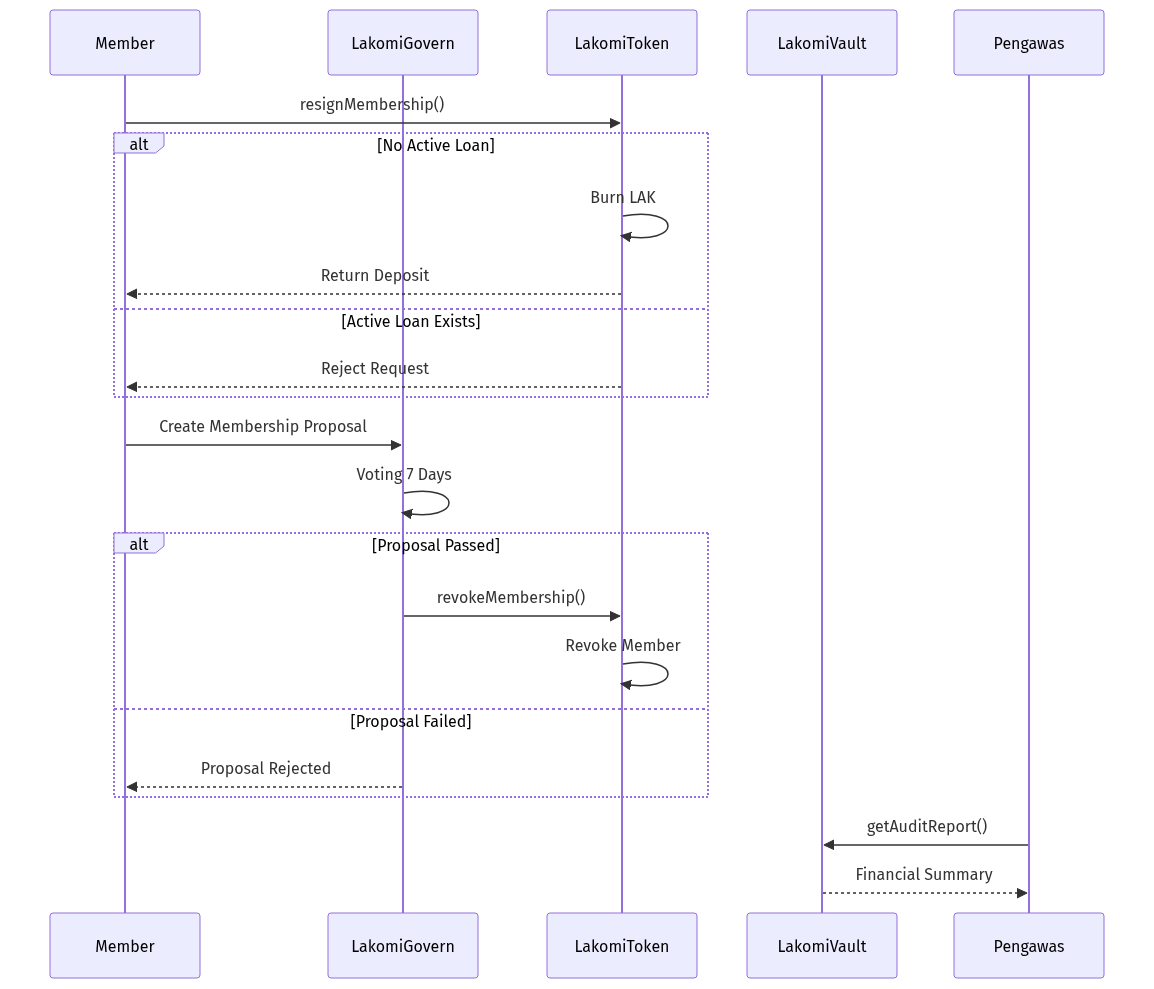
\includegraphics[width=0.75\textwidth]{figures/swimlane-cabut.png}
\caption{Diagram Alir Skenario 4: Pencabutan Keanggotaan dan Audit Pengawas}
\label{fig:swimlane-4}
\end{figure}

\begin{enumerate}
	\item Anggota mengajukan pengunduran diri melalui \texttt{resignMembership()}. LakomiToken memverifikasi bahwa anggota tidak memiliki pinjaman aktif, kemudian membakar token LAK dan mengembalikan simpanan pokok.
	\item Untuk pencabutan paksa, anggota menginisiasi proposal MEMBERSHIP melalui LakomiGovern dengan target anggota yang akan dicabut keanggotaannya.
	\item Proposal melalui siklus pemungutan suara standar (7 hari, kuorum 67\%). Jika lolos dan tidak diveto, LakomiGovern memanggil \texttt{revokeMembership()} pada LakomiToken.
	\item Pengawas melakukan audit keuangan melalui \texttt{getPengawasAuditReport()} pada LakomiVault yang menampilkan ringkasan: total aset dalam IDRX, saldo simpanan pokok/wajib/sukarela, dana cadangan, akumulasi pendapatan bunga, dan daftar pinjaman aktif.
	\item Audit pengawas memastikan bahwa dana \textit{vault} sesuai dengan kewajiban simpanan anggota dan cadangan wajib, setiap ketidakcocokan dapat ditindaklanjuti melalui proposal tata kelola.
	\item Pengawas juga dapat memeriksa riwayat distribusi SHU untuk memverifikasi bahwa alokasi telah sesuai dengan \textit{basis points} yang ditetapkan melalui tata kelola.
\end{enumerate}

\subsection{Skenario 5: Distribusi SHU dan Klaim Anggota}

\begin{figure}[H]
\centering
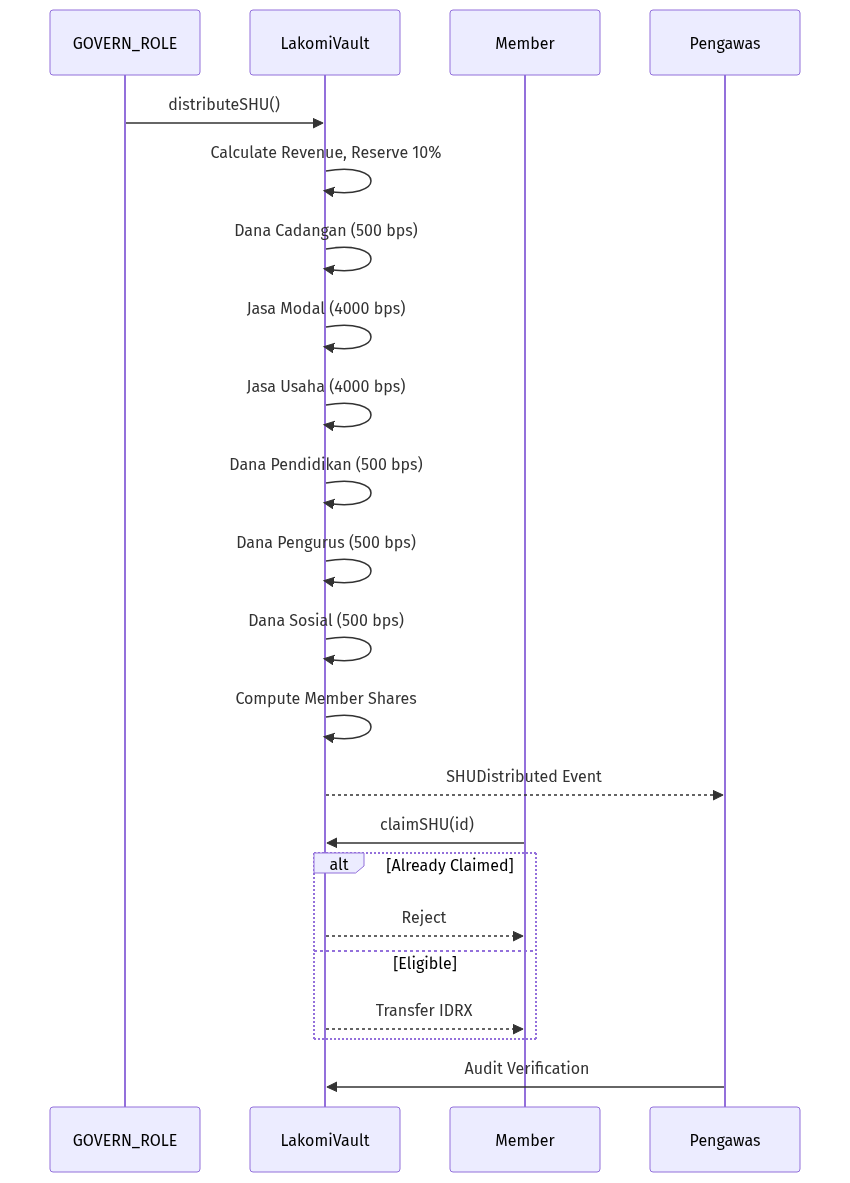
\includegraphics[width=0.75\textwidth]{figures/swimlane-shu.png}
\caption{Diagram Alir Skenario 5: Distribusi SHU dan Klaim Anggota}
\label{fig:swimlane-5}
\end{figure}

\begin{enumerate}
	\item GOVERN\_ROLE memanggil \texttt{distributeSHU()} pada LakomiVault setelah periode akuntansi (setiap 365 hari atau setelah RAT tahunan).
	\item Sistem menghitung SHU yang dapat didistribusikan: 10\% dari total pendapatan (\texttt{accumulatedRevenue}) disisihkan sebagai cadangan operasional, sisanya didistribusikan.
	\item SHU dialokasikan ke enam kategori berdasarkan \textit{basis points}: Dana Cadangan (500 bps), Jasa Modal (4000 bps), Jasa Usaha (4000 bps), Dana Pendidikan (500 bps), Dana Pengurus (500 bps), Dana Kesejahteraan Sosial (500 bps).
	\item Jasa Modal dan Jasa Usaha dihitung secara pro-rata berdasarkan \textit{shares} masing-masing anggota, memastikan distribusi yang proporsional terhadap kontribusi.
	\item Setiap anggota memanggil \texttt{claimSHU(id)} untuk mengklaim bagian SHU-nya. Sistem memverifikasi bahwa anggota belum mengklaim distribusi yang sama dan mentransfer IDRX dari \textit{vault}.
	\item Pengawas dapat memverifikasi seluruh proses melalui \textit{event} \texttt{SHUDistributed} yang dipancarkan dan laporan \texttt{getPengawasAuditReport()}.
\end{enumerate}

\section{Perbandingan Arsitektur dengan Sistem Lain}

Untuk mengontekstualisasikan kontribusi arsitektur Lakomi, bagian ini membandingkan pendekatan sistem dengan tiga model sistem yang relevan: koperasi konvensional, \textit{Decentralized Autonomous Organization} (DAO) berbasis \textit{token-weighted voting}, dan \textit{blockchain cooperative} yang telah diusulkan dalam literatur. Perbandingan dirangkum dalam Tabel~\ref{tab:arsitektur-comparison}.

\begin{table}[H]
\centering
\caption{Perbandingan Arsitektur Lakomi dengan Sistem Lain}
\label{tab:arsitektur-comparison}
\footnotesize
\resizebox{\textwidth}{!}{\begin{tabular}{p{0.20\textwidth}p{0.24\textwidth}p{0.24\textwidth}p{0.26\textwidth}}
\toprule
\textbf{Aspek} & \textbf{Koperasi Konvensional} & \textbf{DAO Token-Weighted} & \textbf{Lakomi (Penelitian Ini)} \\
\midrule
Model Keanggotaan & Formulir manual, verifikasi administrasi & \textit{Permissionless}, siapa pun dapat bergabung & Registrasi mandiri dengan simpanan pokok sebagai syarat \\
\midrule
Hak Suara & Satu anggota satu suara (manual) & Proporsional terhadap kepemilikan token & Satu anggota satu suara (otomatis, on-chain) \\
\midrule
Sistem Simpanan & Buku manual, tiga jenis simpanan & Tidak ada simpanan terstruktur & Tiga jenis simpanan (pokok, wajib, sukarela) on-chain \\
\midrule
Distribusi SHU & Kalkulasi manual, rawan kesalahan & Proporsional terhadap \textit{staking} & Enam kategori SHU dengan basis poin terkonfigurasi \\
\midrule
Transparansi & Akses terbatas pada laporan periodik & Seluruh transaksi publik di \textit{ledger} & Seluruh transaksi publik + fungsi audit pengawas \\
\midrule
Pengawasan & Pengawas eksternal periodik & Tidak ada mekanisme pengawasan formal & Veto pengawas + laporan keuangan on-chain \\
\midrule
Keamanan Dana & Rekening bank, otorisasi manual & \textit{Smart contract}, risiko \textit{reentrancy} & RBAC + ReentrancyGuard + \textit{timelock} \\
\midrule
Kepatuhan Regulasi & Bergantung pada kepatuhan manual & Tidak dirancang untuk regulasi spesifik & 26 ketentuan UU 25/1992 terpetakan ke fungsi on-chain \\
\midrule
Insentif Kontribusi & Tidak ada mekanisme formal & \textit{Staking} memengaruhi hak suara & \textit{Tier} kontribusi menentukan LTV tanpa memengaruhi suara \\
\bottomrule
\end{tabular}}
\end{table}

Arsitektur Lakomi menjembatani kesenjangan antara koperasi konvensional dan DAO dengan pendekatan \textit{dual-track}: (1) \textit{track} demokratis yang memastikan setiap anggota memiliki hak suara setara sesuai Pasal 24(3) UU 25/1992, dan (2) \textit{track} kontribusi yang memberikan insentif finansial melalui \textit{tier} LTV berbasis simpanan tanpa mengompromikan prinsip kesetaraan suara. Pemisahan ini merupakan kontribusi desain utama yang membedakan Lakomi dari DAO berbasis token (\textit{token-weighted voting}) yang berpotensi menghasilkan plutokrasi, serta dari koperasi konvensional yang tidak memiliki mekanisme insentif kontribusi terstruktur.

Dibandingkan dengan \textit{blockchain cooperative} yang diusulkan dalam literatur, seperti El Amine dan Sari (2024) yang berfokus pada registri properti dan Saito dan Rose (2023) yang menggunakan reputasi untuk tata kelola, Lakomi adalah sistem pertama yang secara sistematis memetakan seluruh ketentuan UU 25/1992 ke dalam \textit{smart contract} yang dapat dieksekusi. Pendekatan pemetaan regulasi langsung ini memastikan bahwa kepatuhan bukan merupakan fitur tambahan (\textit{afterthought}) properti bawaan dari arsitektur sistem.

\section{Pengujian}

Pengujian dilakukan dalam dua kategori utama: pengujian fungsional \textit{smart contract} dan analisis gas (\textit{gas analysis}). Pengujian fungsional bertujuan memverifikasi bahwa seluruh 26 ketentuan UU 25/1992 yang telah dipetakan ke dalam fungsi \textit{smart contract} berjalan sesuai spesifikasi. Analisis gas bertujuan mengukur kelayakan operasional sistem dari sisi konsumsi komputasi blockchain.

\subsection{Pengujian Fungsional Smart Contract}

Pengujian fungsional dilakukan menggunakan \textit{framework} Hardhat pada lingkungan DChain. Metode pengujian yang digunakan adalah \textit{unit testing} berbasis skenario, di mana setiap ketentuan UU 25/1992 diverifikasi melalui satu atau lebih skenario pengujian yang mencakup \textit{happy path} (jalur normal) dan \textit{edge cases} (kasus batas). Setiap skenario pengujian mengeksekusi fungsi \textit{smart contract} secara langsung dan memverifikasi hasilnya melalui \textit{assertion} terhadap perubahan \textit{state} on-chain, \textit{event} yang dipancarkan, dan nilai kembalian fungsi.

Pengujian mencakup tujuh area fungsional utama yang dipetakan ke ketentuan UU 25/1992:

\begin{enumerate}
	\item Pendaftaran dan Keanggotaan (Pasal 5(1), 17--18, 19--21, 19(2), 30(2)(b)), Skenario pengujian meliputi: pendaftaran anggota mandiri; verifikasi \texttt{isRegisteredMember} setelah pendaftaran; penolakan pendaftaran ganda; pengunduran diri melalui \texttt{resignMembership()}; dan pencabutan keanggotaan melalui tata kelola dengan \texttt{revokeMembership()}.
	
	\item Satu Anggota Satu Suara (Pasal 24(3)), Skenario pengujian meliputi: verifikasi bahwa dua anggota dengan saldo token berbeda sama-sama mengembalikan \texttt{getVotingPower() = 1}; dan verifikasi bahwa alamat yang tidak terdaftar ditolak saat mencoba membuat proposal atau memberikan suara.
	
	\item Simpanan (Pasal 41(2)), Skenario pengujian meliputi: pembayaran simpanan pokok satu kali dengan verifikasi \texttt{simpananPokok[member] > 0} dan penolakan pembayaran ganda; pembayaran simpanan wajib periodik dengan verifikasi pencatatan yang akurat; dan penyetoran simpanan sukarela dengan perhitungan \textit{shares} yang proporsional.
	
	\item Tata Kelola dan Kuorum (Pasal 24(2), 26--27), Skenario pengujian meliputi: pembuatan proposal oleh anggota terdaftar; pemungutan suara dengan tiga opsi (For, Against, Abstain); verifikasi kuorum 67\%, dengan tiga anggota dan dua suara \textit{For}, proposal dinyatakan lolos; verifikasi bahwa proposal dengan partisipasi di bawah kuorum dinyatakan \textit{defeated}; penjadwalan RAT tahunan melalui \texttt{scheduleAnnualRAT()} dengan pencegahan RAT ganda dalam satu periode; dan verifikasi bahwa RAT hanya dapat dijadwalkan satu kali per 365 hari.
	
	\item Pengawas (Pasal 38--39(2)), Skenario pengujian meliputi: pemberian peran PENGAWAS\_ROLE kepada akun yang ditunjuk; veto proposal oleh pengawas dengan verifikasi bahwa \texttt{proposalVetoed} bernilai \texttt{true}; penolakan veto oleh akun non-pengawas; dan akses pengawas terhadap laporan keuangan melalui \texttt{getPengawasAuditReport()} yang menampilkan ringkasan aset, simpanan, dana cadangan, dan pendapatan.
	
	\item Distribusi SHU (Pasal 45(1--2)), Skenario pengujian meliputi: akumulasi pendapatan dari bunga pinjaman; distribusi SHU oleh GOVERN\_ROLE ke enam kategori (Cadangan 5\%, Jasa Modal 40\%, Jasa Usaha 40\%, Pendidikan 5\%, Pengurus 5\%, Kesejahteraan Sosial 5\%); klaim SHU oleh anggota dengan verifikasi jumlah yang diterima sesuai dengan \textit{shares}; dan pencegahan klaim ganda pada distribusi yang sama.
	
	\item Pinjaman (Pasal 41(2)(a), 44, Permenkop 8/2023 Pasal 43--45), Skenario pengujian meliputi: pengajuan pinjaman dengan perhitungan \textit{loan-to-value} berbasis \textit{tier} kontribusi (30\%, 50\%, 70\%); verifikasi kecukupan agunan 25\% dalam token LAK; penguncian agunan saat pencairan; \textit{auto-approval} untuk pinjaman di bawah 200 IDRX; persetujuan manual oleh APPROVER\_ROLE untuk pinjaman besar; pelunasan penuh dengan pembukaan agunan; dan verifikasi bahwa bunga dialirkan ke LakomiVault sebagai \texttt{accumulatedRevenue}.
\end{enumerate}

Sebagai ilustrasi, Penggalan Kode~\ref{lst:test-register} dan~\ref{lst:test-vote} menyajikan implementasi skrip pengujian untuk dua area fungsional utama. Seluruh skrip pengujian tersedia pada repositori GitHub penelitian.

\begin{lstlisting}[language={}, caption={Skrip Pengujian: Pendaftaran Anggota (Pasal 5(1) UU 25/1992)}, label={lst:test-register}, basicstyle=\ttfamily\scriptsize, breaklines=true]
describe("Pasal 5(1): Open & Voluntary Membership", function () {
 it("should allow self-registration", async function () {
 await token.connect(alice).registerMember();
 expect(await token.isRegisteredMember(alice.address)).to.be.true;
 expect(await token.memberCount()).to.equal(1);
 });

 it("should mint 100 LAK tokens on registration", async function () {
 await token.connect(alice).registerMember();
 expect(await token.balanceOf(alice.address)).to.equal(LAK(100));
 });

 it("should not allow duplicate registration", async function () {
 await token.connect(alice).registerMember();
 await expect(
  token.connect(alice).registerMember()
 ).to.be.revertedWith("Already registered");
 });
});
\end{lstlisting}

\begin{lstlisting}[language={}, caption={Skrip Pengujian: Satu Anggota Satu Suara (Pasal 24(3) UU 25/1992)}, label={lst:test-vote}, basicstyle=\ttfamily\scriptsize, breaklines=true]
describe("Pasal 24(3): One Member One Vote", function () {
 it("each member has 1 voting power", async function () {
 expect(await token.getVotingPower(alice.address)).to.equal(1);
 expect(await token.getVotingPower(bob.address)).to.equal(1);
 expect(await token.getVotingPower(dave.address)).to.equal(0);
 });

 it("non-members cannot vote", async function () {
 await expect(
  govern.connect(dave).castVote(0, 1)
 ).to.be.reverted;
 });
});
\end{lstlisting}

\begin{lstlisting}[language={}, caption={Skrip Pengujian: Simpanan (Pasal 41(2) UU 25/1992)}, label={lst:test-simpanan}, basicstyle=\ttfamily\scriptsize, breaklines=true]
describe("Pasal 41: Simpanan (Deposits)", function () {
 it("should pay Simpanan Pokok (one-time join fee)", async function () {
 await usdc.connect(alice).approve(await vault.getAddress(), USDC(100));
 await vault.paySimpananPokok(alice.address);
 expect(await vault.simpananPokok(alice.address)).to.equal(USDC(100));
 expect(await vault.hasPaidSimpananPokok(alice.address)).to.be.true;
 });

 it("should not pay Simpanan Pokok twice", async function () {
 await usdc.connect(alice).approve(await vault.getAddress(), USDC(200));
 await vault.paySimpananPokok(alice.address);
 await expect(vault.paySimpananPokok(alice.address)).to.be.reverted;
 });

 it("should pay Simpanan Wajib (periodic mandatory)", async function () {
 await usdc.connect(alice).approve(await vault.getAddress(), USDC(200));
 await vault.paySimpananPokok(alice.address);
 await usdc.connect(alice).approve(await vault.getAddress(), USDC(10));
 await vault.connect(alice).paySimpananWajib();
 expect(await vault.simpananWajibTotal(alice.address)).to.equal(USDC(10));
 });
});
\end{lstlisting}

\begin{lstlisting}[language={}, caption={Skrip Pengujian: Pengawas (Pasal 38 UU 25/1992)}, label={lst:test-pengawas}, basicstyle=\ttfamily\scriptsize, breaklines=true]
describe("Pasal 38: Pengawas (Supervisor)", function () {
 it("pengawas can veto a proposal", async function () {
 await token.connect(alice).registerMember();
 await token.connect(bob).registerMember();
 await govern.connect(alice).createProposal(
  "Test proposal", 0, await vault.getAddress(), 0, "0x"
 );
 await govern.vetoProposal(0);
 const state = await govern.state(0);
 expect(state).to.equal(8);
 });

 it("non-pengawas cannot veto", async function () {
 await token.connect(alice).registerMember();
 await govern.connect(alice).createProposal(
  "Test", 0, await vault.getAddress(), 0, "0x"
 );
 await expect(govern.connect(alice).vetoProposal(0)).to.be.reverted;
 });
});
\end{lstlisting}

\begin{lstlisting}[language={}, caption={Skrip Pengujian: Distribusi SHU (Pasal 45(1--2) UU 25/1992)}, label={lst:test-shu}, basicstyle=\ttfamily\scriptsize, breaklines=true]
describe("Pasal 45: SHU Distribution", function () {
 it("should distribute SHU by shares", async function () {
 await usdc.connect(alice).approve(await vault.getAddress(), USDC(1000));
 await vault.connect(alice).receiveRevenue(USDC(1000));
 await vault.distributeSHU();
 expect(await vault.shuDistributionCount()).to.equal(1);
 const dist = await vault.shuDistributions(0);
 expect(dist.totalAmount).to.be.gt(0);
 });

 it("should not claim SHU twice", async function () {
 await usdc.connect(alice).approve(await vault.getAddress(), USDC(1000));
 await vault.connect(alice).receiveRevenue(USDC(1000));
 await vault.distributeSHU();
 await vault.connect(alice).claimSHU(0);
 await expect(vault.connect(alice).claimSHU(0)).to.be.reverted;
 });
});
\end{lstlisting}

\begin{lstlisting}[language={}, caption={Skrip Pengujian: Pinjaman (Pasal 44 UU 25/1992 dan Permenkop 8/2023)}, label={lst:test-loan}, basicstyle=\ttfamily\scriptsize, breaklines=true]
describe("LakomiLoans: Basic Flow", function () {
 it("should request and auto-approve small loan", async function () {
 await usdc.connect(alice).approve(await loans.getAddress(), USDC(1000));
 await loans.connect(alice).requestLoan(
  USDC(100), 30n * 24n * 3600n, "Emergency"
 );
 const loan = await loans.getLoan(0);
 expect(loan.status).to.equal(1);
 });

 it("should repay loan and unlock collateral", async function () {
 await usdc.connect(alice).approve(await loans.getAddress(), USDC(1000));
 await loans.connect(alice).requestLoan(
  USDC(100), 30n * 24n * 3600n, "Emergency"
 );
 await loans.disburse(0);
 const loan = await loans.getLoan(0);
 const totalOwed = loan.principal + loan.interest;
 await usdc.connect(alice).approve(await loans.getAddress(), totalOwed);
 await loans.connect(alice).repayInFull(0);
 expect((await loans.getLoan(0)).status).to.equal(3);
 });
});
\end{lstlisting}

Seluruh hasil pengujian fungsional disajikan dan dibahas secara rinci pada Bab~\ref{ch4}.

\subsection{Analisis Gas}

Analisis gas dilakukan untuk mengukur konsumsi komputasi setiap operasi koperasi pada lingkungan DChain. Pengukuran dilakukan menggunakan \textit{gas reporter} Hardhat yang mencatat konsumsi gas untuk setiap fungsi \textit{smart contract} yang dieksekusi. Operasi yang diukur meliputi:

\begin{enumerate}
	\item Deployment kontrak, Biaya \textit{deployment} satu kali untuk masing-masing dari empat kontrak: LakomiToken, LakomiVault, LakomiGovern, dan LakomiLoans.
	\item Pendaftaran anggota (\texttt{registerMember()}), Operasi yang melibatkan \textit{minting} token dan penulisan \textit{state} keanggotaan.
	\item Pembayaran simpanan (\texttt{paySimpananPokok()}), Operasi penulisan saldo simpanan dan \textit{shares}.
	\item Pengajuan pinjaman (\texttt{requestLoan()}), Operasi yang melibatkan perhitungan LTV, verifikasi agunan, dan penulisan \textit{state} pinjaman.
	\item Pemungutan suara (\texttt{castVote()}), Operasi pencatatan suara pada proposal.
	\item Distribusi SHU (\texttt{distributeSHU()}), Operasi distribusi dana ke enam kategori dengan perhitungan \textit{basis points}.
	\item Pelunasan pinjaman (\texttt{repayInFull()}), Operasi transfer dana, pembukaan agunan, dan pencatatan pendapatan bunga.
\end{enumerate}

Hasil analisis gas disajikan dan dibahas pada Bab~\ref{ch4}.

\subsection{Pengujian Imutabilitas}

Pengujian imutabilitas dilakukan untuk memverifikasi bahwa sistem memenuhi prinsip \textit{append-only} dan \textit{non-transferable} yang merupakan fondasi kepercayaan dalam sistem berbasis blockchain. Pengujian ini mencakup:

\begin{enumerate}
	\item Non-transferabilitas Token Keanggotaan, Verifikasi bahwa setiap upaya untuk mentransfer token LAK antar akun akan ditolak (\textit{reverted}) karena \texttt{transfersEnabled = false}. Pengujian dilakukan dengan memanggil fungsi \texttt{transfer()} standar ERC-20 dan memverifikasi bahwa transaksi gagal.
	\item Imutabilitas Data Simpanan, Verifikasi bahwa setelah pembayaran simpanan dicatat dalam \texttt{simpananPokok} dan \texttt{simpananWajib}, data tersebut tidak dapat diubah atau dihapus oleh pihak mana pun kecuali melalui fungsi yang telah ditentukan (misalnya, \texttt{refundSimpananPokok()} pada saat pengunduran diri).
	\item Imutabilitas Riwayat Proposal, Verifikasi bahwa proposal yang telah dieksekusi atau diveto tetap tercatat dalam \textit{state} kontrak dan tidak dapat dimodifikasi. Setiap perubahan status proposal (dari Active ke Succeeded/Defeated/Vetoed) bersifat final dan tidak dapat dikembalikan.
	\item Imutabilitas Catatan Pinjaman, Verifikasi bahwa riwayat pinjaman, termasuk pengajuan, persetujuan, pencairan, pembayaran, dan pelunasan, tercatat secara permanen dalam \texttt{Loan} struct dan tidak dapat dihapus.
\end{enumerate}

Seluruh hasil pengujian fungsional, analisis gas, dan pengujian imutabilitas disajikan secara rinci pada Bab~\ref{ch4}.
